% =============================================================================
\section{GHZM states}
% =============================================================================

We also perform mesoscopic Schr\"odinger cat state simulations, corresponding to recent ion-trap experiments with $M$ qubits.
These states violate a genuine multipartite Bell inequality, which means that it is impossible to confine the Bell violation to a microscopic part of the state.
Such inequalities require the measurement of all possible correlation functions at the highest order available.
We find two distinct scaling laws for the total computational difficulty, as measured by the number of samples required to obtain a given sampling error.

To understand the ultimate scaling properties of probabilistic sampling methods, we have also simulated higher order correlations that violate multipartite Bell inequalities.
These are found in quantum states that display Bell violations with $M$ observers, not just two.
The most well-known examples are the multimode entangled Greenberger-Horne-Zeilinger-Mermin (\abbrev{ghzm}) states~\cite{Greenberger1989,Mermin1990}, corresponding to ``Schr\"odinger Cat'' states.
We therefore considered \abbrev{ghzm} states which describe $M$ spin-$\frac{1}{2}$ particles or qubits:
\begin{eqn}
\label{eqn:bell-ineq:ghz:state}
    \vert\Phi\rangle
    = \frac{1}{\sqrt{2}} \left(
        \ket{\uparrow\ldots\uparrow}
        + e^{i\phi} \ket{\downarrow\ldots\downarrow}
    \right).
\end{eqn}
Here $\ket{\uparrow}$ and $\ket{\downarrow}$ denote spin-up or spin-down particles in the $z$-direction.
As well as being of deep significance in quantum physics, such mesoscopic states have been generated in recent ion-trap experiments~\cite{Rowe2001,Leibfried2005,Monz2011}.

Quantum paradoxes are obtained on measuring an operator $\hat{A}$ which is defined as a linear combination of $2^{M}$ distinct $M$-th order correlation functions:
\begin{eqn}
\label{eqn:bell-ineq:ghz:operator}
    \hat{A}
    = \prod_{j=1}^{M} \left(
            \hat{\sigma}_j^x
            + i \hat{\sigma}_j^y
        \right),
\end{eqn}
where $s_j \in {-1, +1}$, and $\hat{\sigma}_j^x$ and $\hat{\sigma}_j^y$ are the Pauli spin operators acting on the $j$-th qubit.
We consider the constraints imposed by a \abbrev{lhv} on the expectation $A_{\lambda}(\phi) \equiv \langle \Phi(\phi) \vert \hat{A} \vert \Phi(\phi) \rangle_\lambda$ (where $\langle \rangle_{\lambda}$ stands for the expectation under \abbrev{lhv} assumptions), as compared to the predictions for these expectations given by quantum mechanics, $A_{\mathrm{QM}}(\phi) \equiv \langle \Phi(\phi) \vert \hat{A} \vert \Phi(\phi) \rangle$.

Mermin~\cite{Mermin1990} originally proved that for the phase difference $\phi=\pi/2$, \abbrev{qm} predicts that
\begin{eqn}
    \Imag A_{\mathrm{QM}}(\pi / 2)
    = 2^{M - 1},
\end{eqn}
while the \abbrev{lhv} bounds are
\begin{eqn2}
    \Imag A_{\lambda}(\pi / 2) & \le 2^{M/2},\quad & M\,\mathrm{is\,even}, \\
    \Imag A_{\lambda}(\pi / 2) & \le 2^{(M-1)/2},\quad & M\,\mathrm{is\,odd}.
\end{eqn2}
Ardehali~\cite{Ardehali1992} then proved that for $\phi=\pi$, the predictions are
\begin{eqn}
    -\Real A_{\mathrm{QM}}(\pi)
    = 2^{M - 1},
\end{eqn}
and
\begin{eqn2}
    -\Real A_{\lambda}(\pi) & \le 2^{(M-1)/2},\quad & M\,\mathrm{is\,even}, \\
    -\Real A_{\lambda}(\pi) & \le 2^{M/2},\quad & M\,\mathrm{is\,odd}.
\end{eqn2}
Here we transformed the original expressions given by Ardehali to the equivalent ones that use our definition of the target operator~\eqnref{bell-ineq:ghz:operator}.

It is clear that the Mermin inequalities are stronger for odd $M$, and the Ardehali ones are stronger for even $M$ (in particular, for $M = 2$ the Mermin inequalities are not even violated by \abbrev{qm}).
Therefore for our sampling tests in this section we will use the strongest of two inequalities, and the corresponding phase difference in the \abbrev{ghzm} state, for every $M$:
\begin{eqn2}
    F & = -\Real A_{\lambda}(\pi),\quad & M\,\mathrm{is\,even},\\
    F & = \Imag A_{\lambda}(\pi / 2),\quad & M\,\mathrm{is\,odd}.
\end{eqn2}
Consequently, for \abbrev{qm} and \abbrev{lhv} predictions we get the uniform \abbrev{qm} prediction $F_{\mathrm{QM}} = 2^{M - 1}$ and the inequality
\begin{eqn}
\label{eqn:bell-ineq:ghz:general-ineq}
    F_{\lambda} \le 2^{(M-1)/2}.
\end{eqn}
The relative violation can thus be made arbitrarily big to compensate for any imperfections in the measurements.


% =============================================================================
\subsection{Positive-P representation}
% =============================================================================

The na\"ive approach to the sampling of the state~\eqnref{bell-ineq:ghz:state} is to use the P-representation, as we did in the previous section.
In general, spin-up and spin-down states are represented as $\ket{\uparrow}\equiv\ket{10}$ and $\ket{\downarrow}\equiv\ket{01}$, where $\ket{0}$ and $\ket{1}$ are number states, which allows for straightforward application of Pauli spin operators.

But for our particular choice of the target operator~\eqnref{bell-ineq:ghz:operator}, we can choose a simplified representation, which will halve the dimensionality of the resulting phase space: $\ket{\uparrow}\equiv\ket{0}$ and $\ket{\downarrow}\equiv\ket{1}$.
Since every term of $\hat{A}$ contains only one spin operator per qubit, it can be expressed in terms of creation and annihilation operators by replacing the spin operators with
\begin{eqn}
    \hat{\sigma}_j^x = \hat{a}_j + \hat{a}_j^\dagger,\quad
    \hat{\sigma}_j^y = \frac{1}{i} (\hat{a}_j - \hat{a}_j^\dagger),
\end{eqn}
from which the equivalent function of $\balpha$ and $\bbeta$ in P-representation immediately follows.

The P-representation of the target state is obtained with the canonical formula~\cite{Drummond1980}
\begin{eqn}
    P[\hat{\rho}]
    = \left( \frac{1}{4\pi^2} \right)^M
        \exp\left(
            -\frac{|\balpha -\bbeta^*|^2}{4}
        \right)
        \bra{\frac{1}{2} \left( \balpha + \bbeta^* \right)}
        \hat{\rho}
        \ket{\frac{1}{2} \left( \balpha + \bbeta^* \right)},
\end{eqn}
which for $\rho \equiv \ket{\Phi} \bra{\Phi}$ gives
\begin{eqn}
    P
    = \frac{1}{2 \pi^{2M}} e^{-|\bmu|^2} e^{-|\blambda^2|}
        \left|
            \prod_{j=1}^M \lambda_j + 1
        \right|^2,
\end{eqn}
where we have peformed the variable change~\eqnref{bell-ineq:cooperative:mu-lambda}
\begin{eqn}
    \bmu = \frac{\balpha - \bbeta^*}{2},\quad
    \blambda = \frac{\balpha + \bbeta^*}{2}.
\end{eqn}

The sampling is performed using the rejection method with bounding $P$ as
\begin{eqn}
    P
    \le \frac{1}{2 \pi^{2M}} e^{-|\bmu|^2} e^{-|\blambda^2|}
        \left( \prod_{j=1}^M |\lambda_j|^2 + 1 \right).
\end{eqn}
Therefore $P$ can be sampled using a combination of independent samples from Gaussian and gamma distributions, and then conditionally rejecting samples, as described in the previous section.

The phase space in this representation has $4M$ dimensions.
This can be further improved by using a specialized representation, allowing us to reduce the sampling error significantly, thus making the states with larger values of $M$ accessible for sampling.


% =============================================================================
\subsection{SU(2)-Q representation}
% =============================================================================

The theoretical derivation of the SU(2)-Q representation was performed by L.~E.~C.~Rosales-Z\'arate.
In this subsection we we will briefly describe the framework of the representation, and apply it to our target state.

The positive-P representation does not impose any restrictions on the phase space, including the number states with population more than $1$ in the calculation of moments.
While it does not affect the calculated observable, it does increase the sampling error.
For the cases when we know that the system consists of binary states, more suitable representations exist.

We will consider a Q-representation~\cite{Husimi1940} for SU(2) coherent states~\cite{Arecchi1972,Zhang1990}:
\begin{eqn}
    \kket{\zvec}
    = \prod_{j=1}^{M} \left(
            \ket{\downarrow}_j + z_j \ket{\uparrow}_j
        \right),
\end{eqn}
where $z_j$ are complex numbers.
The SU(2)-Q function is the expectation value of the density operator over the SU(2) coherent states, and is defined explicitly in a normalized form as:
\begin{eqn}
    Q[\hat{\rho}]
    = \left(
        \prod_{j=1}^M \frac{2}{\pi (1 + |z_j|^2)^3}
    \right) \bbra{\zvec} \hat{\rho} \kket{\zvec}.
\end{eqn}
For the target \abbrev{ghzm} state~\eqnref{bell-ineq:ghz:state} the function takes form of a probability distribution
\begin{eqn}
    Q
    = \frac{1}{2} \prod_{j=1}^M
        \frac{2}{\pi (1 + |z_j|^2)^3}
        \left|
            \prod_{j=1}^M z_j + e^{-i \phi}
        \right|^2
\end{eqn}

The sampling is again performed using the rejection method with bounding $Q$ as
\begin{eqn}
    Q
    \le \frac{1}{2} \prod_{j=1}^M
        \frac{2}{\pi (1 + |z_j|^2)^3}
        \left(
            \prod_{j=1}^M |z_j|^2 + 1
        \right),
\end{eqn}
and using the inverse sampling on both terms.
The expectation of $\hat{A}$ can be shown to be
\begin{eqn}
    A_{\mathrm{SU(2)-Q}}
    = \int
        6^M \prod_{j=1}^M \frac{z_j^*}{1 + |z_j|^2}
        Q(\zvec) \upd^2 \zvec.
\end{eqn}


% =============================================================================
\subsection{Results}
% =============================================================================

\begin{figure}
    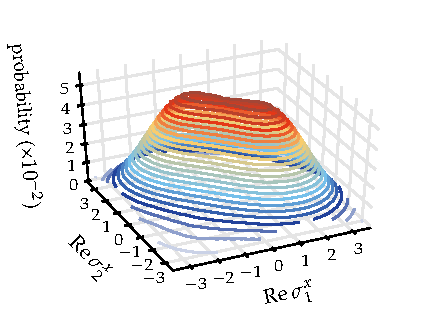
\includegraphics{figures_generated/bell/distribution_P1.pdf}%
    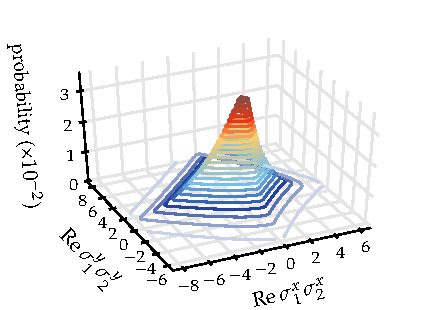
\includegraphics{figures_generated/bell/distribution_P2.pdf}\\
    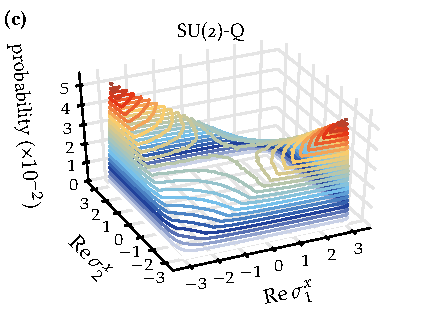
\includegraphics{figures_generated/bell/distribution_Q1.pdf}%
    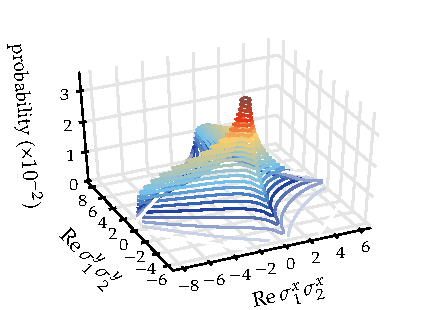
\includegraphics{figures_generated/bell/distribution_Q2.pdf}

    \caption{
    Correlations for the different parts of the inequality~\eqnref{bell-ineq:ghz:general-ineq-M2}, in case of \textbf{(a, b)} positive-P and \textbf{(c, d)} SU(2)-Q representations, $10^8$ samples.}

    \label{fig:bell-ineq:ghz:correlations}
\end{figure}

The difference between the positive-P and SU(2)-Q representations (and their difference from \abbrev{lhv} theories) can be illustrated on the inequality~\eqnref{bell-ineq:ghz:general-ineq} for $M = 2$:
\begin{eqn}
\label{eqn:bell-ineq:ghz:general-ineq-M2}
    - \langle \hat{\sigma}_1^x \hat{\sigma}_2^x \rangle_{\lambda}
    + \langle \hat{\sigma}_1^y \hat{\sigma}_2^y \rangle_{\lambda}
    \le \sqrt{2}.
\end{eqn}
The real parts of the correlations in this expression for both representations used are plotted in~\figref{bell-ineq:ghz:correlations}.

The main feature of quasiprobability representations is apparent: neither of them limits the value of $\Real \sigma_1^x$ or $\Real \sigma_2^x$ to the range $[-1, 1]$, as would happen in a \abbrev{lhv} theory.
This means that the Bell theorem does not apply to these results, because the sampled values differ from their physical equivalents.
Moreover, the plots for the SU(2)-Q show that in this representation the correlations are more peaked, and also do not have exponential tails as the ones in the positive-P representation.
This, in addition to the reduced phase space dimensionality, allows the sampling with SU(2)-Q representation for high values of $M$.

\begin{figure}
    \centerline{%
    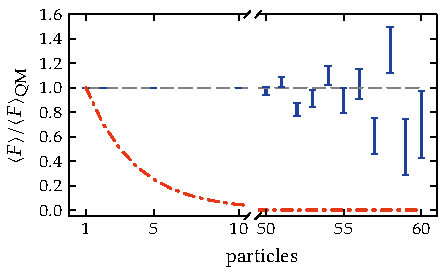
\includegraphics{figures_generated/bell/ghz_violations.pdf}%
    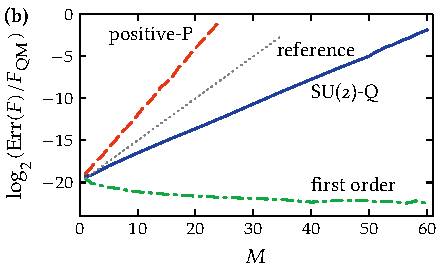
\includegraphics{figures_generated/bell/ghz_errors.pdf}}

    \caption{
    Violations of the inequality~\eqnref{bell-ineq:ghz:general-ineq} for multi-particle \abbrev{ghzm} states.
    \textbf{(a)} Blue bars shos the expectation $F$ simulated using the SU(2)-Q representation, with the length of the bars corresponding to the sampling error.
    The values of expectations and errors are normalized by the quantum mechanical prediction for the corresponding $M$.
    The horizontal grey dashed line gives the quantum prediction.
    The red dash-dotted line is the \abbrev{lhv} prediction, which gives a Bell violation when the expectation $F$ is above this line.
    \textbf{(b)} Relative sampling errors for $F$ simulated using the positive-P (red dashed line) and SU(2)-Q (blue solid line) representations.
    Sampling errors for a first order correlation (total number of ``spin-ups'') in the SU(2)-Q representation are plotted as the green dashed line.
    The dotted reference line $\log_2 \mathrm{error} \propto M$ shows the point at which the sampling errors would give scaling properties as slow as an experimental measurement.}

    \label{fig:bell-ineq:ghz:violation}
\end{figure}

The results for test of the inequality~\eqnref{bell-ineq:ghz:general-ineq} using the SU(2)-Q representation are shown in~\figref{bell-ineq:ghz:violation}.
We have used a \abbrev{gpu} to sample the distribution and calculate the required correlation for the values of $M$ up to $60$.
